\documentclass{article}

\usepackage[utf8]{inputenc}
\usepackage{graphicx}
\usepackage{hyperref}


\title{De Révolution à Evolution \\ Création d'un jeu vidéo sur les thèmes de l'écologie et de la transition énergétique}
\date{16-02-2018}
\author{Niels Lachat}

\begin{document}
        \pagenumbering{gobble}
        \maketitle
        \newpage
        \pagenumbering{arabic}

        \section{Introduction}
        Le but de ce travail de maturité était de créer un jeu vidéo abordant les thématiques de l'environnement et de la transition énergétique. Le genre du jeu de gestion a été choisi pour démontrer les principes économiques de la transition énergétique.
        
        \section{Concept du jeu}
        \subsection{Développement du concept}
        
        

        \begin{figure}[h]
                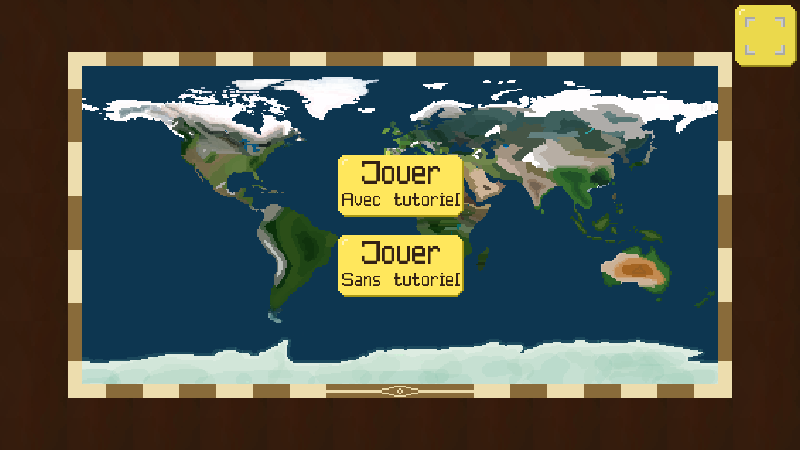
\includegraphics[width=\linewidth]{../images/mainMenu}
                \caption{Menu principal du jeu}
                \label{fig:mainMenu}
        \end{figure}

        Figure \ref{fig:mainMenu}

        \href{https://www.latex-tutorial.com/tutorials/figures/}{Lien vers le tuto}



\end{document}
